		% article example for classicthesis.sty
\documentclass[12pt,a4paper]{article} % KOMA-Script article scrartcl
\usepackage{lipsum}
\usepackage{url}
\usepackage[nochapters]{classicthesis} % nochapters
%%%%%
\usepackage{geometry} % Required to change the page size to A4
\geometry{left=1.5cm,right=1.5cm,top=2.5cm,bottom=2.5cm}
\geometry{a4paper} % Set the page size to be A4 as opposed to the default US Letter
\usepackage{amssymb}

\usepackage{graphicx}
\usepackage{subfig}
% Required for including pictures
\usepackage{amsthm}
\usepackage{float} % Allows putting an [H] in \begin{figure} to specify the exact location of the figure
%\usepackage{wrapfig} % Allows in-line images such as the example fish picture
\usepackage{amsmath}
\usepackage{hyperref}
\usepackage{listings}
\usepackage{alltt}


% Theorem Styles
\newtheorem{theorem}{Theorem}[section]
\newtheorem{lemma}[theorem]{Lemma}
\newtheorem{proposition}[theorem]{Proposition}
\newtheorem{corollary}[theorem]{Corollary}
% Definition Styles
\theoremstyle{definition}
\newtheorem{definition}{Definition}[section]
\newtheorem{example}{Example}[section]
\theoremstyle{remark}
\newtheorem{remark}{Remark}

%%%%%%%%%%%%%%%%%%%%%%%%%%%%%%%%%%%%%%%%%%%%%%%%
%%%%%%%%%%%%%%%%%%%%%%%%%%%%%%%%%%%%%%%%%%%%%%%%
\begin{document}
	\title{\rmfamily\normalfont\spacedallcaps{ECE 1747 : Parallel Programming - Assignment 1}}
	\author{\spacedlowsmallcaps{Chen Sun}, \spacedlowsmallcaps{Student Number: 1001418799}\\
	\spacedlowsmallcaps{Jiayue Zhang}, \spacedlowsmallcaps{Student Number: 1003555146}	}
	\date{} % no date
	
	\maketitle
	
	%    \begin{abstract}
	%        \noindent\lipsum[1] Just a test.\footnote{This is a footnote.}
	%    \end{abstract}
	
	%    \tableofcontents
\section{Background Introduction}
The current common issue for servers of on-line games is the load management problem. The problem is that given a game consisting of M regions assigned to N servers, we need to find a proper way to relocate regions to servers such that we can balance the server load and decrease inter-sever communication. This report is based on the algorithm comparison between `static' and `dynamic' schemes in several scenarios. The problem here is that we want to balance server load by replicating existing game world partitions across several servers and decrease inter-server communication by maintaining locality of adjacent regions. 

\vspace{3mm}

One existing solutions for this problem is static partitioning for example, row or column based partition. The static partitioning limits cross-server interactions between
players, and exposes the division of the world to players. We have also dynamic load balancing algorithms. 
The dynamic load management algorithm enables us to better handle transient crowding by adaptively dispersing or aggregating regions from servers in response to quality of service violations.


\vspace{3mm}

In this report, we use SimMud, a massively multiplayer game simulator to implement and evaluate the Dynamic Uniform Load Spread -  ``Spread'' method. 
We analyze the performance of the “static” vs. “dynamic” schemes in the following two scenarios:
\begin{itemize}
	\item [(a)] There is no active quest and the players are moving more or less randomly,
	\item [(b)] There is an active quest and as a result all the players are concentrated in one area the map. 
\end{itemize}
 The rest of this report is organized
 as follows: Section 2 introduces the related background of SimMud and implementation. In section 3, we  analyzes the simulation results and compare the performance of the static vs. spread scheme. Section 4 concludes this report.

\section{SimMud Implementation}
We use the SimMud provided and add some test variables in the three-staged loop. In ``src/server/WorldUpdateModule.cpp'', we have implemented test variables to examine the following interested terms for each thread:
\begin{itemize}
	\item Number of client requests
	\item Time spent on processing clients' requests
	\item Number of client updates
	\item Time sending updates
\end{itemize}

\vspace{3mm}


For the implementation of Simmud, we have listed several simulation parameters in Table 1.
Some parameters of the Map in the config file are changed, such as map size, region size (in number of client-areas-of-interest), blocks and resources. These enlarged parameters may make the synchronization more difficult and make the experiment results distinct.

\begin{center}
	\captionof{table}{Some of the Simulation Parameters}
    \begin{tabular}{ | l | l | l | l | }
    \hline
    Map Size & Block & Resources & Region Size\\ \hline
    48x48 & 100 & 50 & 8x8 \\ \hline
\end{tabular}


\end{center}

\vspace{3mm}



\vspace{3mm}

\section{Simulation Result}
In this section, we compared the performance between static and spread method in two different scenarios. 


\subsection{No Active Quest}
In this part, we stick to the case where the quest is random, hence the flocking effect should be less. 
\subsubsection {Number of players}
	\begin{figure}[!ht]
		\subfloat[Static partition\label{subfig-1:dummy}]{%
			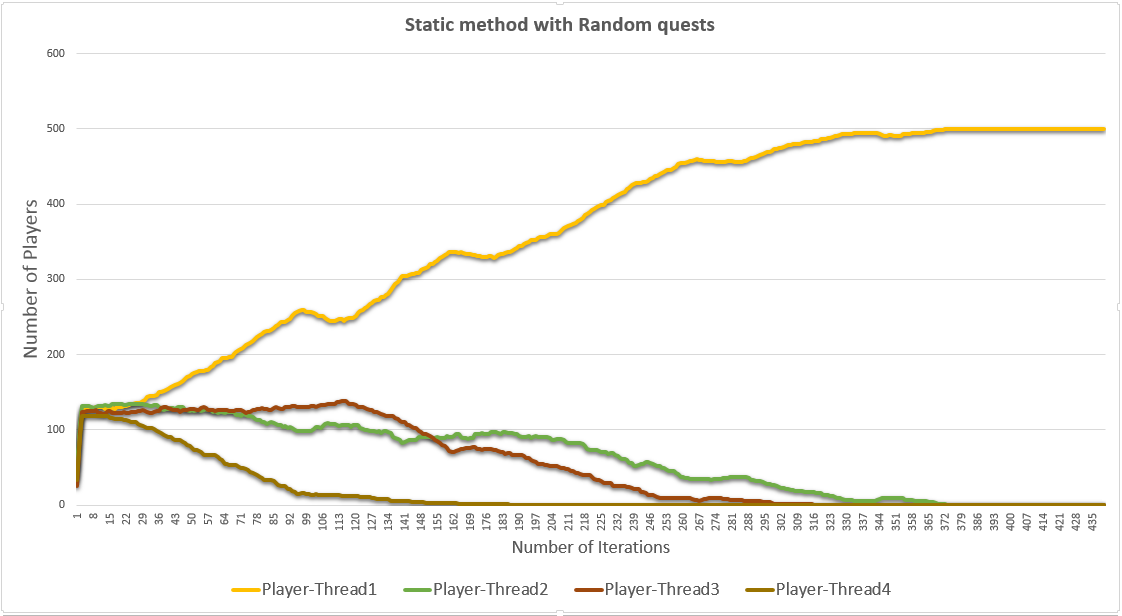
\includegraphics[width=0.45\textwidth]{Static_random_player.png}
		}
		\hfill
		\subfloat[Spread method\label{subfig-2:dummy}]{%
			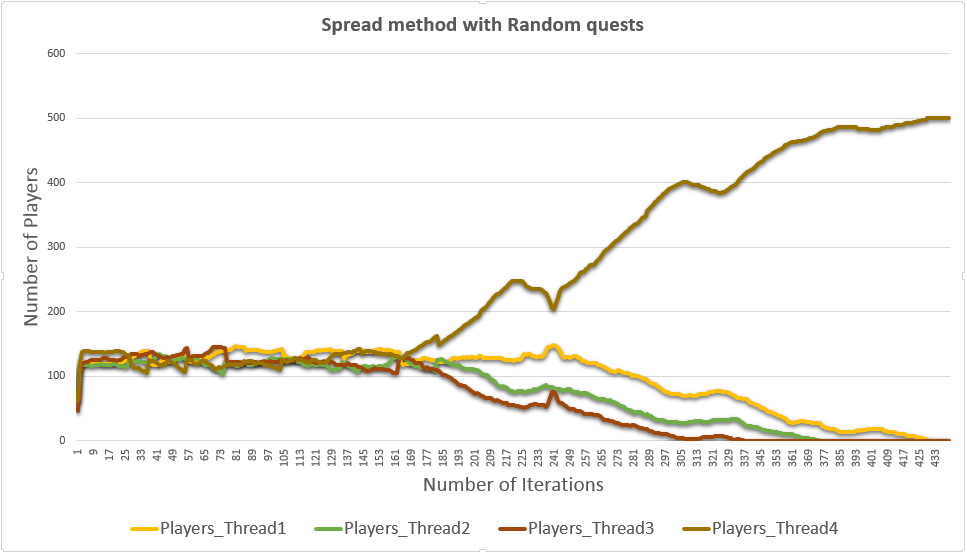
\includegraphics[width=0.45\textwidth]{Player_spread_random.png}
		}
		\caption{Number of Players for each thread in the random quests scenario}
		\label{Player_random}
	\end{figure}
Figure \ref{Player_random} (a) and (b) showed player distribution on each thread for Static and Spread method. 
From the figure, we can see that Static
has uneven distribution of players, especially after 36th iteration and almost all players are concentrated to one Thread after 288th iteration. There is no adjustment after for static method. 
On the other hand, Spread has players allocated in each thread uniformly for most of the time.
After 193th iteration,  distribution of players in spread method started to have uneven behavior. This is much better than static. Further  more, there is obvious attempt of adjustment at 241th  and 329th iteration. 
Unfortunately, after a certain period of time of an active quest, players eventually are gathered into a single
thread. 
We concluded such behavior is due to players are moving to a single region which cannot be
transferred to another thread. 
This is may be due to the simulation region size is not large enough. 
The spread method have better performance according to the player numbers on each thread.


\subsubsection {Number of requests} 
	\begin{figure}[!ht]
		\subfloat[Static partition\label{request1}]{%
			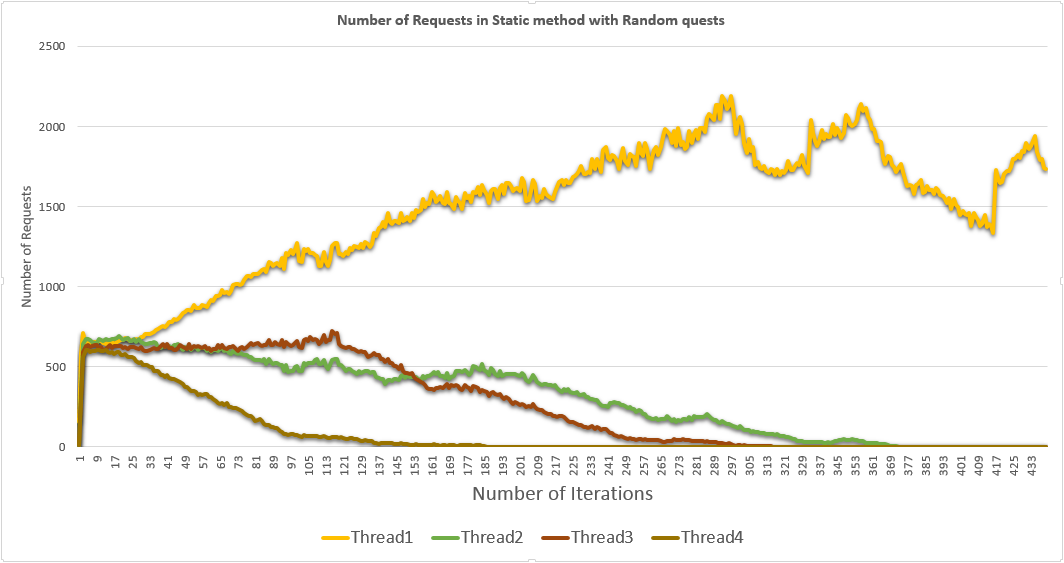
\includegraphics[width=0.45\textwidth]{static_random_request.png}
		}
		\hfill
		\subfloat[Spread method\label{request2}]{%
			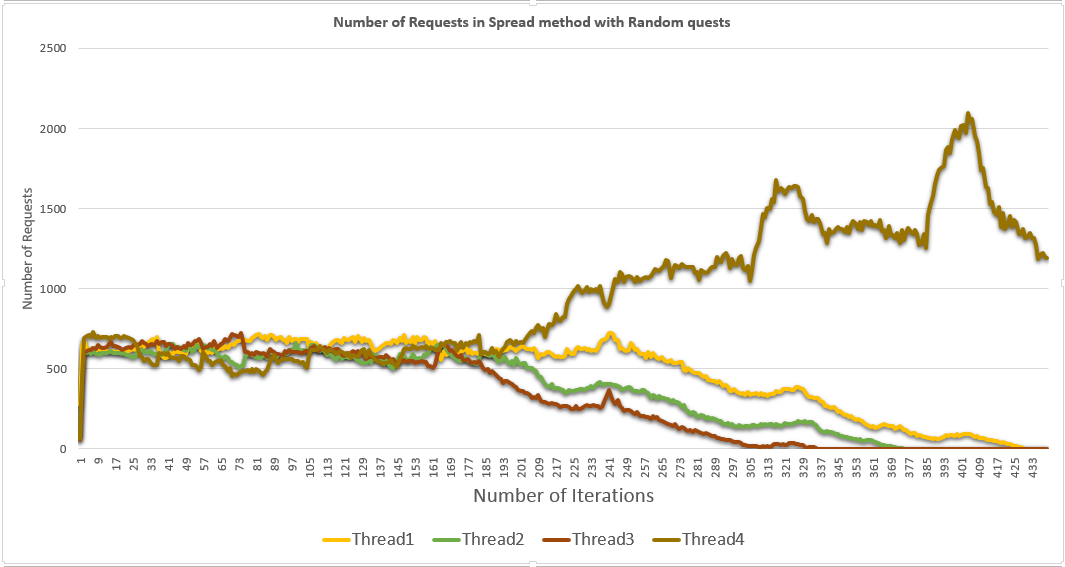
\includegraphics[width=0.45\textwidth]{spread_random_request.png}
		}
		\caption{Number of requests for each thread in the random quests scenario}
		\label{Request_random}
	\end{figure}
Figure \ref{Request_random} (a) and (b) showed the requests per second in each thread for Static and Spread. 
They have shown a strong correlation between the player distribution and request distribution. 
A quest requires the players to move to another region. All the threads in these two schemes deal with approximately 500 requests in no quest phase and after the quests come in, larger amount of requests are sent to Thread 1 in Static and Thread 4 in Spread, which are the destinations.

\subsubsection {Update time comparison} 
	\begin{figure}[!ht]
		\subfloat[Static partition\label{updatetime_random1}]{%
			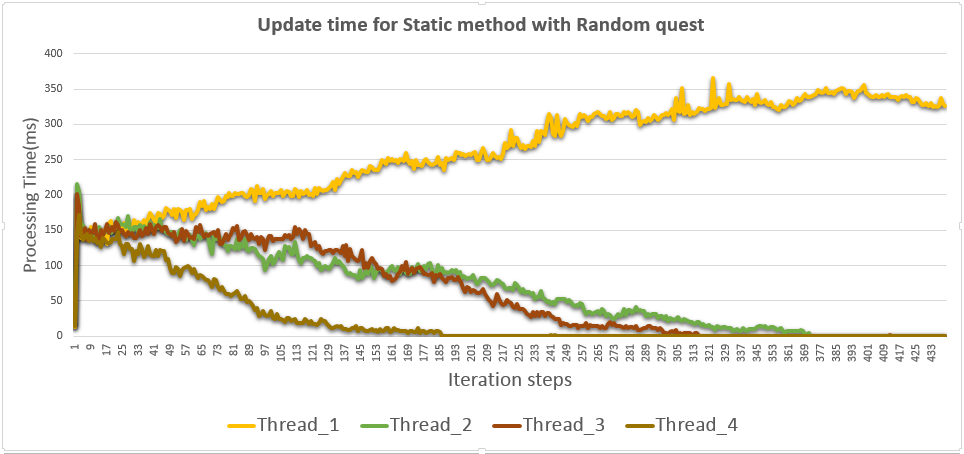
\includegraphics[width=0.45\textwidth]{Update_time_static_random.png}
		}
		\hfill
		\subfloat[Spread method\label{updatetime_random2}]{%
			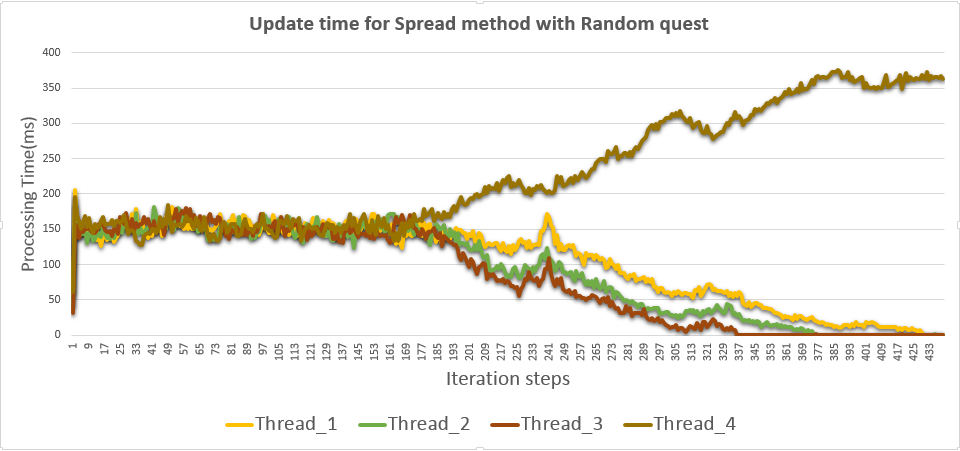
\includegraphics[width=0.45\textwidth]{Update_time_spread_random.png}
		}
		\caption{Update time for each thread in the random quests scenario}
		\label{update_time_random}
	\end{figure}
Similarly, Figure \ref{update_time_random} (a) and (b) showed the update time for each thread in the random quests scenario. The processing time for phase 3 overall, spread method wins over static.



\subsubsection {Number of Updates} 
\begin{figure}[!ht]
	\subfloat[Static partition\label{updates_random1}]{%
		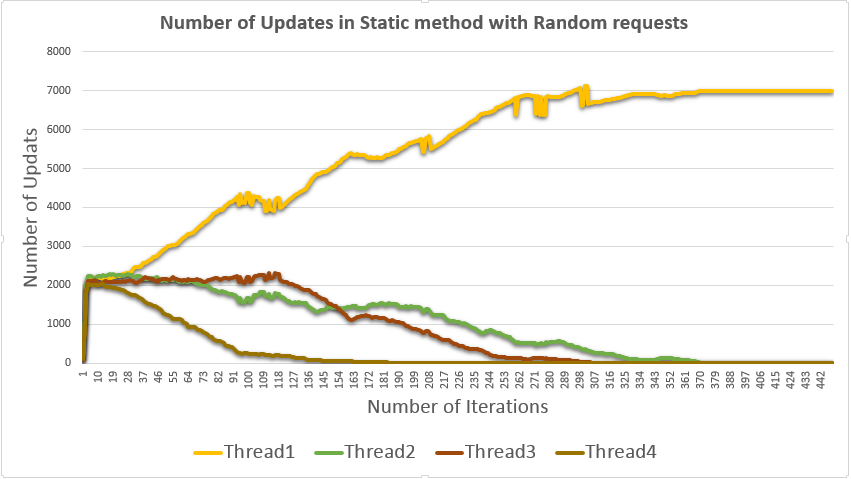
\includegraphics[width=0.45\textwidth]{Updates_static_random.png}
	}
	\hfill
	\subfloat[Spread method\label{updates_random2}]{%
		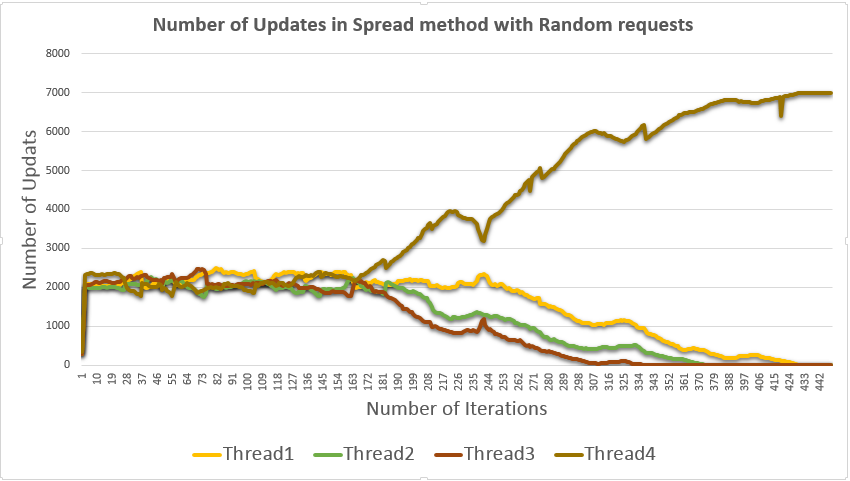
\includegraphics[width=0.45\textwidth]{Updates_spread_random.png}
	}
	\caption{Number of updates for each thread in the random quests scenario}
	\label{updates_random}
\end{figure}
Figure \ref{updates_random} (a) and (b) showed the number of client updates per second in each thread in Static and Spread. 
In Static, more client updates are sent in one thread and it reaches 7k in 279 iterations (28 - 307). But in Spread, the clients
updates to Thread 4 reaches 6k in only 198( 181 - 379) iteration. Server reaches the third stage in the 3-staged loop
that each thread sends back world updates to clients in shorter time in Spread, which proves that Spread
beats Static in processing the quests.



\subsection{Active Quest}
Now we look into the performances in active quest scenario, where the flocking effect would happen way more faster than random quest scenario.
\subsubsection {Number of players}
\begin{figure}[!ht]
	\subfloat[Static partition\label{player_active1}]{%
		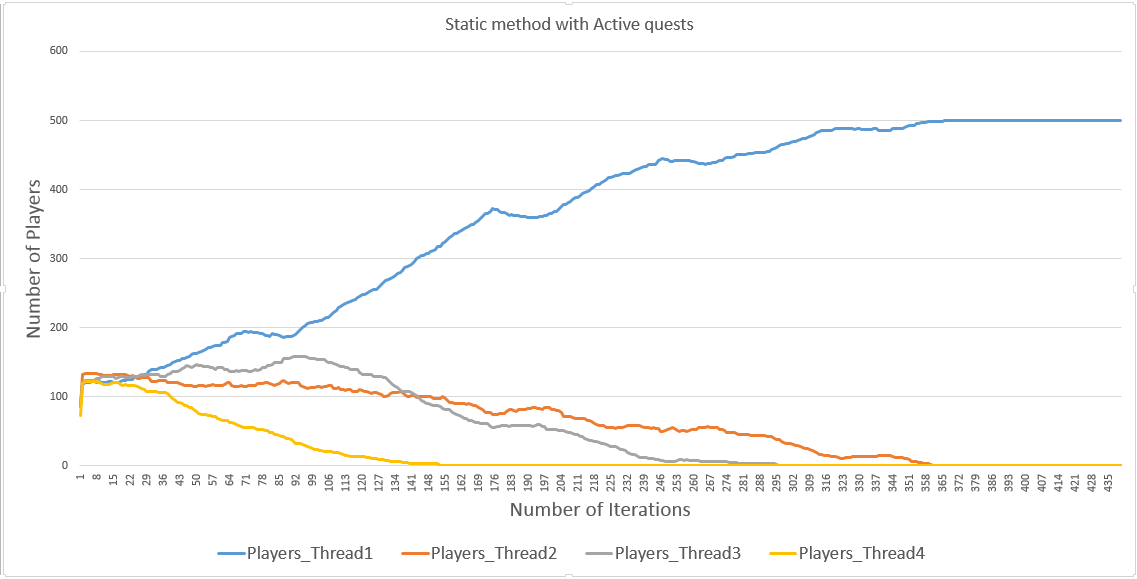
\includegraphics[width=0.45\textwidth]{Static_active_player.png}
	}
	\hfill
	\subfloat[Spread method\label{player_active2}]{%
		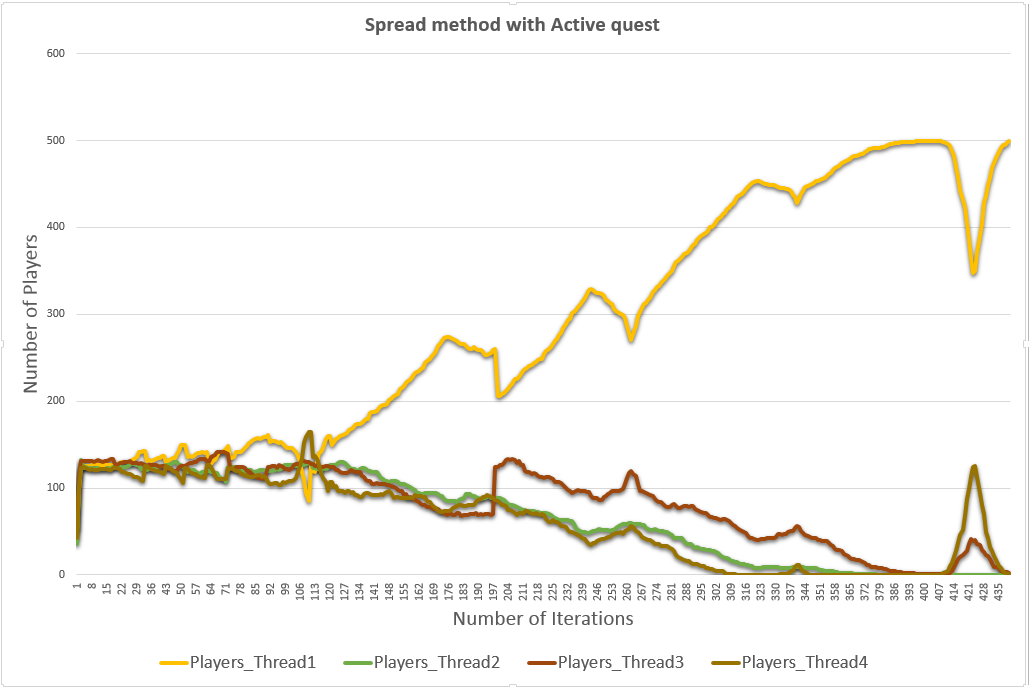
\includegraphics[width=0.45\textwidth]{Player_Spread_active.png}
	}
	\caption{Number of Players for each thread in the active quests scenario}
	\label{Player_random_active}
\end{figure}
Figure \ref{Player_random_active} (a) and (b) compared the player distribution on each thread for Static and Spread method in active quest scenario. 
As we expected, in active quest  scenario, the player flocking behavior happens faster.
We can see that Static
has uneven distribution of players, especially after 29th iteration and almost all players are concentrated to one Thread after 200th iteration. There is no adjustment after for static method. 
On the other hand, for Spread method, player in each thread started to have uneven behavior after 120th iteration, this is quicker than the other scenario. However, there is obvious frequently attempt of adjustment after since in active quest scenario, the player movement is predictable.
We should expect that if the map is large enough and have many regions, the performance of Spread method will be further enhanced.


\subsubsection {Number of requests}
\begin{figure}[!ht]
	\subfloat[Static partition\label{request_active1}]{%
		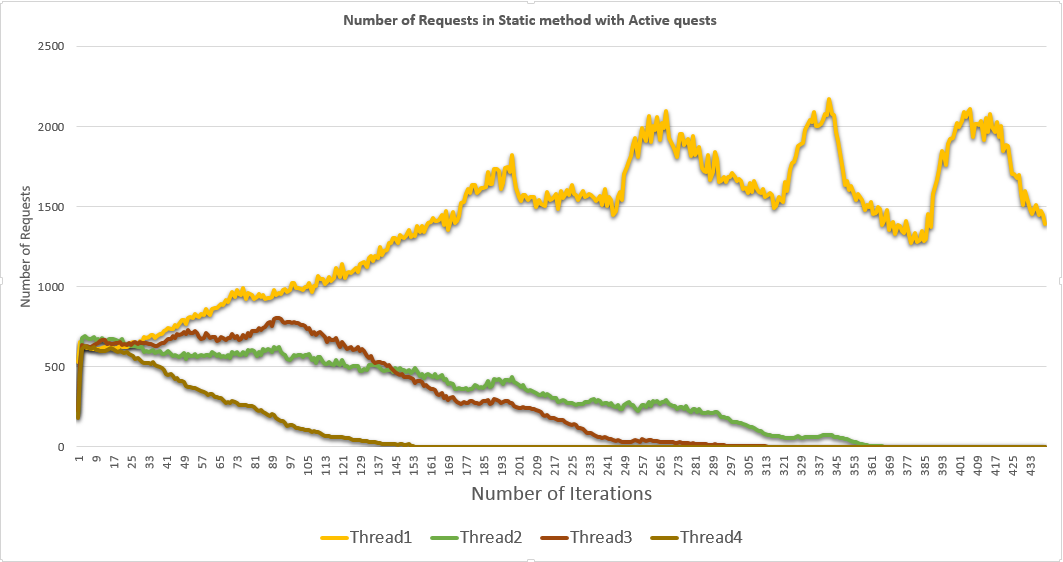
\includegraphics[width=0.45\textwidth]{static_acvtive_request.png}
	}
	\hfill
	\subfloat[Spread method\label{request_active2}]{%
		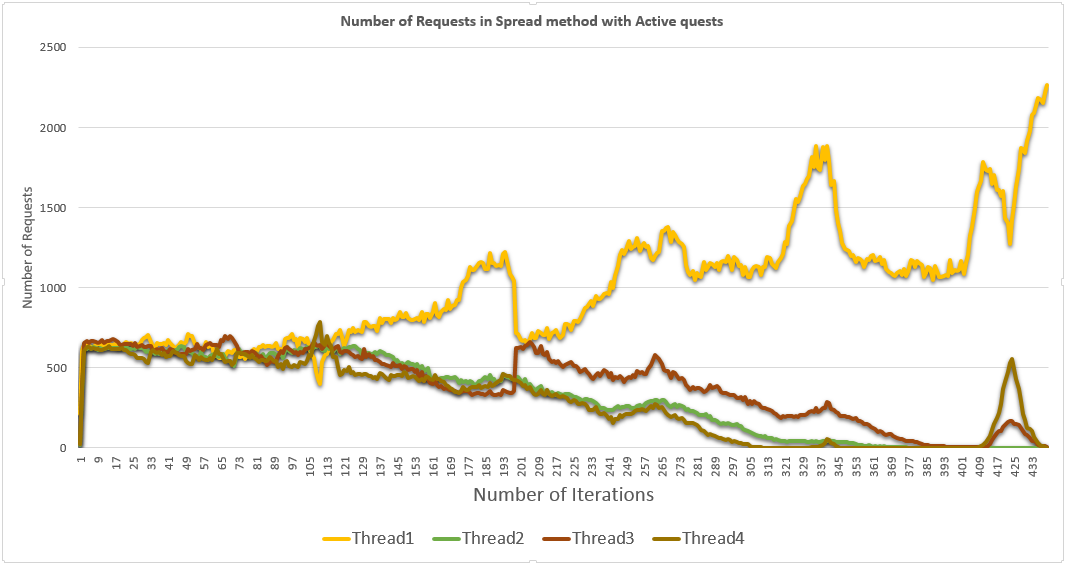
\includegraphics[width=0.45\textwidth]{spread_active_request.png}
	}
	\caption{Number of requests for each thread in the active quests scenario}
	\label{Request_active}
\end{figure}
Similar to the random quest scenario, Figure \ref{Request_active} (a) and (b)  showed the correlation between player distribution and request distribution. There is fluctuations in the distribution because of the active quest. 


\subsubsection {Update time comparison}
\begin{figure}[!ht]
	\subfloat[Static partition\label{updatetime_active1}]{%
		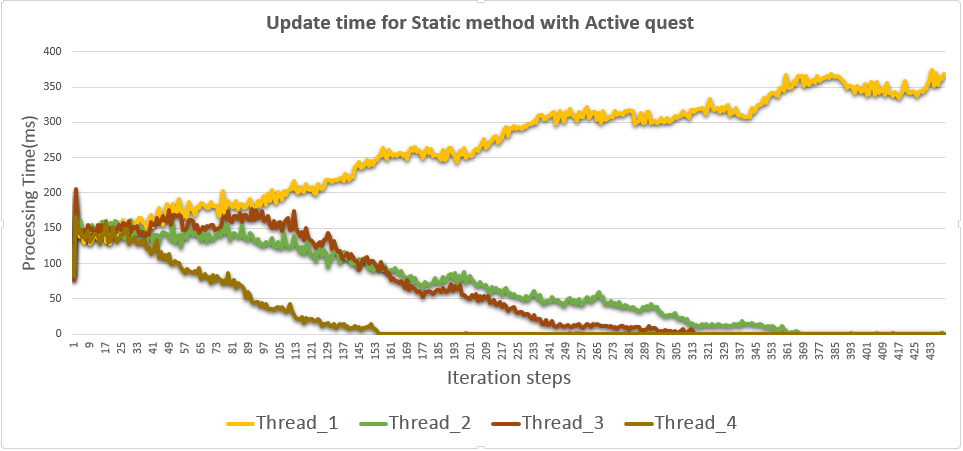
\includegraphics[width=0.45\textwidth]{Update_time_static_active.png}
	}
	\hfill
	\subfloat[Spread method\label{updatetime_active2}]{%
		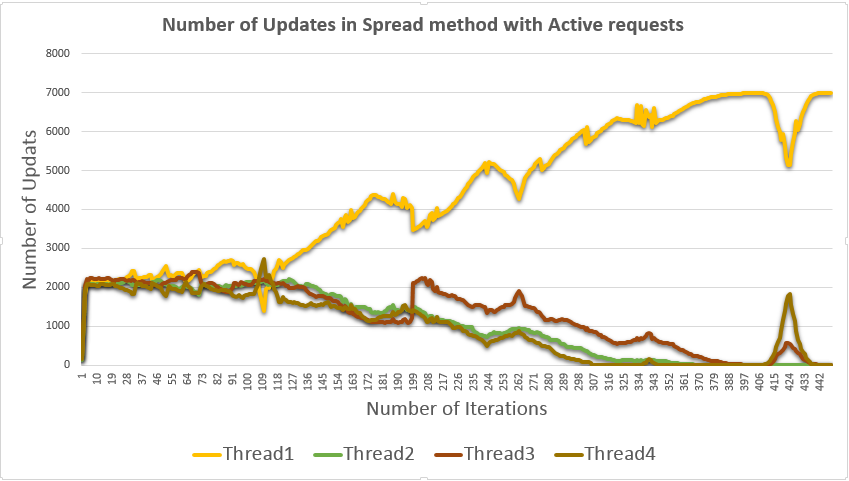
\includegraphics[width=0.45\textwidth]{Updates_Spread_active.png}
	}
	\caption{Update time for each thread in the active quests scenario}
	\label{update_time_active}
\end{figure}
 Figure \ref{update_time_random} (a) and (b) showed the update time for each thread in the active quests scenario. The processing time for phase 3 overall, spread method wins over static.


\subsubsection {Number of Updates}
\begin{figure}[!ht]
	\subfloat[Static partition\label{updates_active1}]{%
		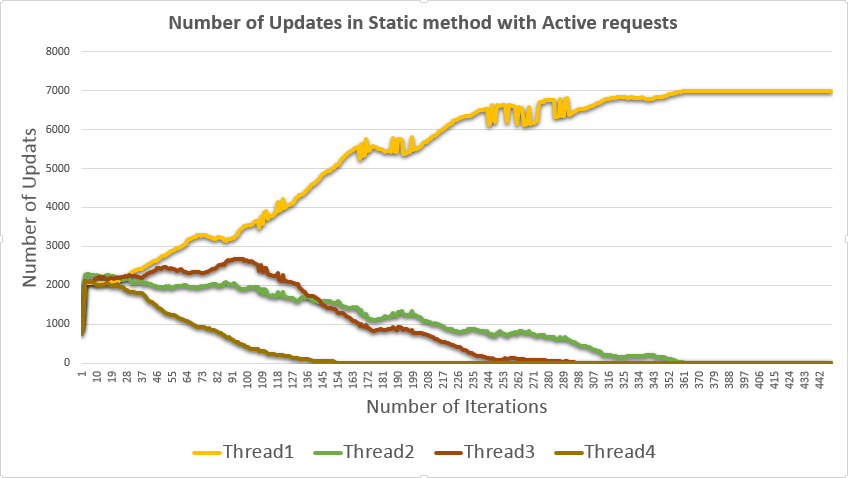
\includegraphics[width=0.45\textwidth]{Updates_static_active.png}
	}
	\hfill
	\subfloat[Spread method\label{updates_active2}]{%
		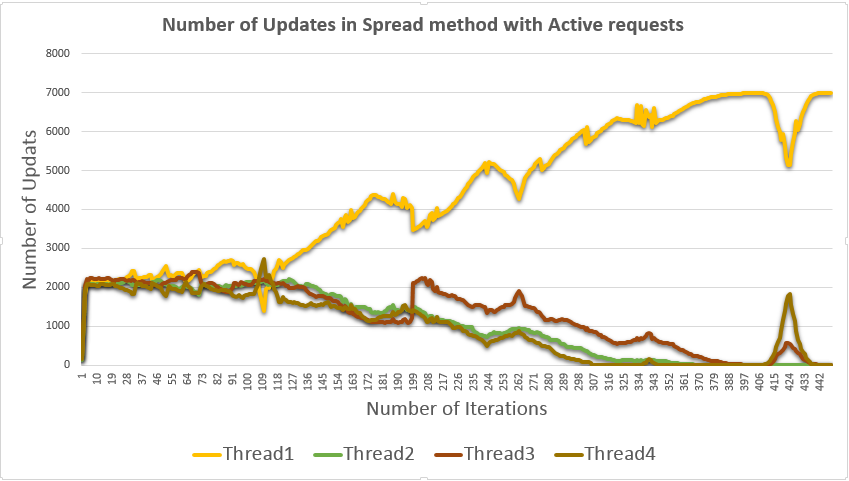
\includegraphics[width=0.45\textwidth]{Updates_Spread_active.png}
	}
	\caption{Number of updates for each thread in the active quests scenario}
	\label{updates_active}
\end{figure}
Figure \ref{updates_active} (a) and (b) showed the number of client updates per second in each thread in Static and Spread in the case where there is active quest. 
In Static, more client updates are sent in one thread and it reaches 7k in 270 iterations (28 - 298). But in Spread, the clients
updates to Thread 4 reaches 6k in only 207 ( 127 - 334) iteration. Server reaches the third stage in the 3-staged loop
that each thread sends back world updates to clients in shorter time in Spread, which proves that Spread
beats Static in processing the quests. However, in the comparison between the random quest scenario, the difference is smaller.




\begin{figure}[htbp]
	\centering
	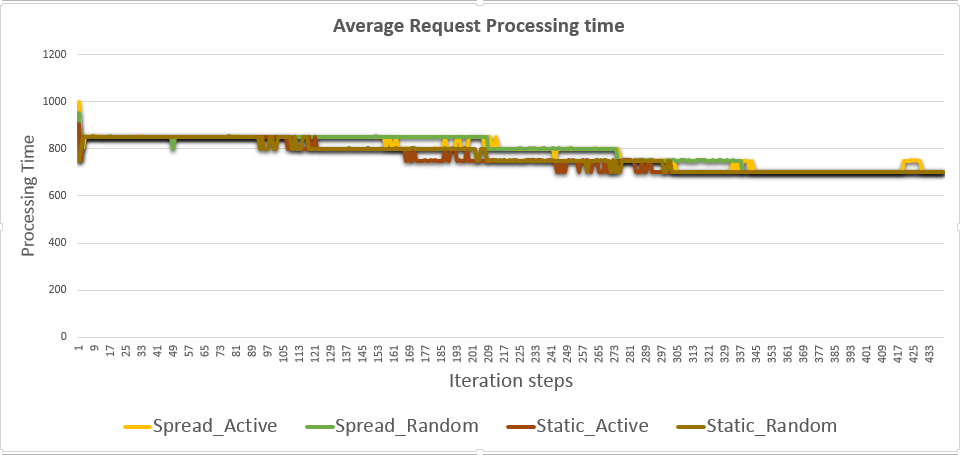
\includegraphics[width=0.65\textwidth]{Average_compare_request_processing_time.png}
	\caption{The comparison of average request processing time}\label{Cpt2_error}
\end{figure}
Figure \ref{Cpt2_error} shows the comparison in the average actual processing time of client requests between Static and
Spread algorithm among the two scenarios. This time is actually only a very small percentage in the entire processing time,
it is reasonable that it is quite similar for those two algorithms. 


\section{Conclusion}
Overall, the performance of spread algorithm outweighs static algorithm from many aspects.
First of all, the Spread method has better performance than Static in the thread/CPU utilization. The load shedding can provide certain adjustment instead static partition cannot.
Further more, Spread algorithm processes more requests/updates than Static in a certain time, hence it is faster. However,
there is one concern in the experiment, the region size. The size will influence load shedding according to which scenario we are in. If the size of the region is too big, then it is hard to assign it to any thread. If the size is too small,
fluctuation happens due to frequent re-assigning overheads. It is quite tricky to choose appropriate region size in order to have better comparison result.




\end{document}